\chapter{Design / Methods Description}
\label{chapter:design}

Concrete header for the proposed design of the thesis's solution

This chapter can contain:
\begin{itemize}
    \item Specification based on the Sections~\ref{sec:sota-summary}
    \item Design
    \item Technologies (can also be/moved in/to Chapter~\ref{chapter:implementation} Implementation)
\end{itemize}

Description how the design works (as much as possible from the below list)
\begin{itemize}
    \item We need to separate our design from our concrete implementation
    
    \item Architecture, Block scheme, Event diagram, Sequence diagram, Algorithms, ...
    
    \item Text description of each blocks and their connections and/or dependencies

    \item Time complexity and memory complexity estimation for each execution step and the whole design. Communication complexity of the design (if any).
\end{itemize}


Figure \ref{fig:dynabook} is about ... description of each blocks
\begin{figure}[h]
    \begin{centering}
    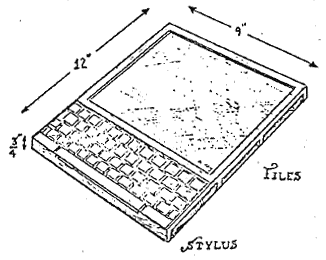
\includegraphics[width=5cm]{assets/images/Dynabook.png}
    \par\end{centering}
    \caption{Architecture/Workflow}
    \label{fig:dynabook}
\end{figure}